\section{Experiments} \label{sec:experiments}

%------------------------------------------------
% Results from Depth diffusion Experiments
%------------------------------------------------
\begin{table*}[t]
\centering
\caption{Results of experiments performed with our depth diffusion model. We alter the model architecture, the method to obtain the variance, the loss formulation, the learning rate schedule, the number of residual blocks per stage and the stochastic depth probability. Underlined parameters depict the change compared to the previous run. The detailed architecture of the models can be found in TABLE \ref{tab:experiment_model_description_depth_diffusion} in the appendix.}
\label{tab:depth_diffusion_ablation}
\begin{tabular}{ l | c c c c c c | r | r | r | r }
\hline
\textbf{Run} & \textbf{Model} & \textbf{Variance} & \textbf{Loss} & \textbf{$L_r$ Schedule} & \textbf{ResBlocks} & \textbf{Stochastic Depth} & \textbf{MAE $\downarrow$} & \textbf{MSE} $\downarrow$ & \textbf{IoU} $\uparrow$  & \textbf{VLB} $\downarrow$ \\ 
\hline
\hline
 dd1 & UNet & fix & simple & \textbf{x} & 2/2/2/2 & 0/0/0/0 & 8.14 & 2.57 & 0.987 & 10.03 \\
 \hline
 dd2 & \underline{UNet3+} & fix & simple & \textbf{x} & 2/2/2/2 & 0/0/0/0 & 9.24 & 2.97 & 0.988 & \textbf{9.72} \\
 dd3 & UNet3+ & \underline{learned} & simple & \textbf{x} & 2/2/2/2 & 0/0/0/0 & 10.83 & 3.21 & 0.987 & 13.00 \\ 
 dd4 & UNet3+ & learned & \underline{P2} & \textbf{x} & 2/2/2/2 & 0/0/0/0 & 8.36 & 1.75 & 0.989 & 14.26 \\ 
 dd5 & UNet3+ & learned & P2 & \underline{\checkmark} & 2/2/2/2 & 0/0/0/0 & 7.70 & 1.58 & \textbf{0.993} & 12.20 \\ 
 dd6 & \underline{UNet} & learned & P2 & \checkmark & 2/2/2/2 & 0/0/0/0 & 7.45 & \textbf{1.48} & 0.990 & 12.39 \\
 dd7 & UNet & learned & \underline{simple} & \checkmark & 2/2/2/2 & 0/0/0/0 & 15.65 & 8.75 & 0.946 & 20.48 \\ 
 dd8 & \underline{UNet3+} & learned & simple & \checkmark & 2/2/2/2 & 0/0/0/0 & 6.16 & 1.64 & \textbf{0.993}  & 17.59 \\
 dd9 & UNet3+ & learned & simple & \checkmark & \underline{2/2/12/2} & 0/0/0/0 & 231.91 & 251.30 & 0.539 & 23.97 \\
 dd10 & UNet3+ & learned & simple & \checkmark & 2/2/12/2 & \underline{0.1/0.1/0.5/0.1} & \textbf{5.79} & \textbf{1.48} & \textbf{0.993} & 16.95  \\
 \hline
\end{tabular}
\end{table*}

\begin{figure*}[t]
  \centering
  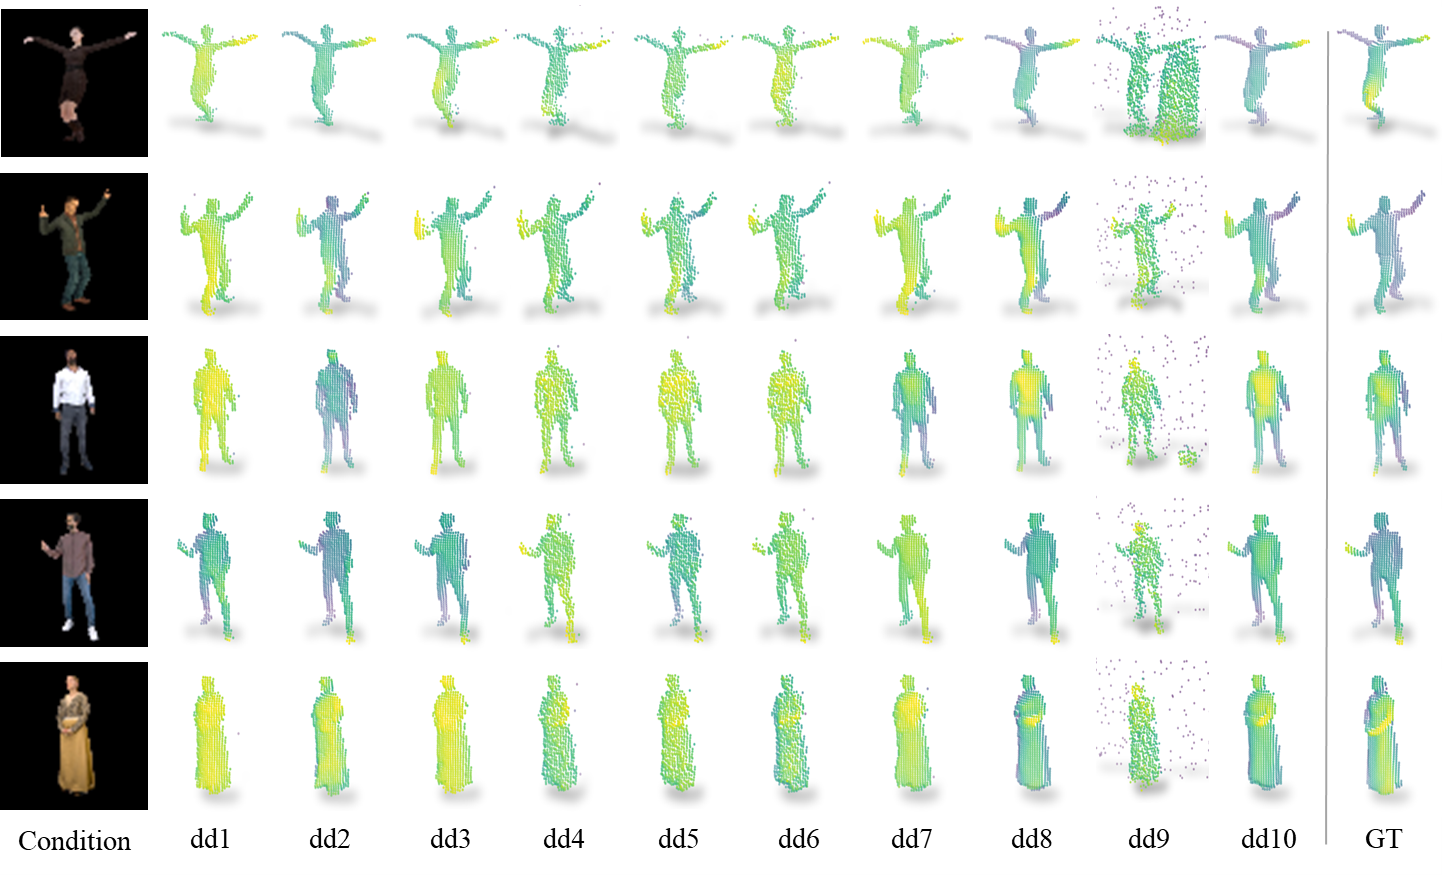
\includegraphics[width=0.99\textwidth]{illustrations/depth_ablation.png}
  \caption{Generated depth maps represented as point clouds $P_{d}$ from our depth diffusion models evaluated in our experiments from TABLE \ref{tab:depth_diffusion_ablation} for each run respectively. To better observe the details, the point clouds' viewpoint has been rotated 10 degrees in azimuth and 10 degrees in elevation. The color map encodes the depth between the min and max value of the depth of each plot, where darker colors indicate higher depth and brighter colors closer depth.}
  \label{fig:depth_ablation}
\end{figure*}
%------------------------------------------------

In this section we perform experiments to validate our design choices. We first run multiple experiments on the conditional depth diffusion network to select various hyperparameters related to model architecture and model training. We incorporate our findings into the conditional depth super-resolution model and find that the best architecture for the depth diffusion is not suitable in terms of resources and performance on the metrics. We hence modify the architecture, investigate on which input modality to condition to and perform an ablation study on the augmentation of the condition input. 
We evaluate our experiments with the following metrics: 
\begin{itemize}
  \item \textbf{MAE} mean average error distance of the ground truth depth $d_{gt}$ and the predicted depth $d_{pred}$ with $d_{gt}, d_{pred} \in \mathbb{R}^{HxWx1}$.
  \begin{equation}
      MAE = \frac{1}{n}\sum_{i=1}^{n}\left|d_{gt}-d_{pred}\right| \cdot 10^{3}
  \end{equation}
  We multiply the result with $10^{3}$. The closer to zero the better.
  \item \textbf{MSE} mean squared error distance of the ground truth depth $d_{gt}$ and the predicted depth $d_{pred}$.
  \begin{equation}
    MSE = \frac{1}{n}\sum_{i=1}^{n}\left(d_{gt}-d_{pred}\right)^2 \cdot 10^{3}
  \end{equation}
  We multiply the result with $10^{3}$. The closer to zero the better.
  \item \textbf{IoU} Intersection over Union calculated over a binary mask $m$ of the ground truth $gt$ and the prediction $p$.  
  \begin{equation}
    IoU = \frac{m_{gt} \cap m_{p}}{m_{gt} \cup m_{p}}, with \; m_{y} = \left\{\begin{array}{ll} 1, & y > \phi \\
         0, & y \le \phi \end{array}\right. 
  \end{equation}
  where $\phi$ is the threshold for the binary mask. We set $\phi=-0.95$ since the depth maps range from [-1,1].
  The closer to 1 the better.
  \item \textbf{VLB} of the negative log-likelihood of the test data set (see \eqref{eq:variational_lower_bound}) reported in bits/dim with base-2 logarithm.
  The smaller the better.
\end{itemize}

As highlighted by \cite{theis_note_2016} the evaluation metrics of generative models are complex and might be misleading especially for high dimensional data like images. High log-likelihood does not imply high sample quality and low log-likelihood does not imply poor samples. Furthermore, an evaluation on samples is claimed to be biased towards overfitting models and favors models of large entropy. We therefore do not rely on a single metric and report the metrics listed above and show samples drawn from the model distribution. 

We further want to highlight the weakness of distance metrics like MSE and MAE since the pixel location is of high importance and even a slight shift of a few pixels of two indistinguishable images leads to a high distance metric, as reported by \cite{theis_note_2016} for a nearest neighbor distance.

All experiments are performed on our test set described in section \ref{subsec:dataset} which contains $\approx 5300$ data samples. 

%%%%%%%%%%%%%%%%%%%%%%%%%%%%%%%%%%%%%%%%%%%%%%%%%%%%%%%%%%%%%%%%%%
% Depth Diffusion Model
%%%%%%%%%%%%%%%%%%%%%%%%%%%%%%%%%%%%%%%%%%%%%%%%%%%%%%%%%%%%%%%%%%
\subsection{Depth Diffusion Model} \label{subsec:experiements_depth_diffusion}
We first investigate the impact of different hyper-parameters on mentioned metrics for our conditional depth diffusion model. Explicitly we perform 10 runs in which we vary the model architecture (UNet vs. UNet3+), the approach for determining the variance (learned range vs. fixed to upper bound $\beta_t$), the loss weighting approach (simple vs. P2), a learning rate schedule (no schedule vs. cosine decay with restart and linear warm-up), the number of residual blocks and the usage of stochastic depth augmentation. A detailed summary of the most important hyper parameters for all runs is listed in TABLE \ref{tab:experiment_model_description_depth_diffusion} in the appendix.

The results for the conditional depth diffusion models are summarized in TABLE \ref{tab:depth_diffusion_ablation} and outputs of the respective models are depicted in Fig. \ref{fig:depth_ablation}. The underlined parameter highlights the changed configuration compared to the previous run. Best results are printed in bold.

Our baseline (Run 1 in TABLE \ref{tab:depth_diffusion_ablation}) is a UNet model (similar to \cite{dhariwal_diffusion_2021}). The variance is not learned but set to $\beta_t$, the upper bound of the reverse diffusion process. We apply the simple loss $L_{simple}$ from equation \eqref{eq:loss_simple} as our training objective and apply no learning rate schedule. 

All runs are trained for 250 epochs using ADAM optimizer with a learning rate $\alpha$ of 4e-5 (exception of Run 5 with $\alpha=6e-5$), $\beta_1=0.9$ and $\beta_2=0.999$. The forward and the reverse diffusion process is performed with $T=600$ time steps and a cosine noise schedule as in \cite{nichol_improved_2021}. We further apply random scaling and shifting augmentation on the RGB input condition. 

Based on the results in TABLE \ref{tab:depth_diffusion_ablation} and the generated images in Fig. \ref{fig:depth_ablation} we consider run dd10 best.

%%%%%%%%%%%%%%%%%%%%%%%%%%%%%%%%%%%%%%%%%%%%%%%%%%%%%%%%%%%%%%%%%%
% Super Resolution Model
%%%%%%%%%%%%%%%%%%%%%%%%%%%%%%%%%%%%%%%%%%%%%%%%%%%%%%%%%%%%%%%%%%
\subsection{Depth Super-Resolution Model} \label{subsec:experiements_superresolution}
We perform various experiments for our super-resolution model. We compare different architectures and ablate the augmentation method. A detailed summary of the most important hyperparameters for all runs is listed in TABLE \ref{tab:experiment_model_description_superres_condition} in the appendix.

First, we investigate the impact of the input condition in combination with the model architecture on lower resolution (64 $\rightarrow$ 128) for performance reasons. We condition the model either on a depth map or an RGB-D image. The intuition is that the RGB channels provide further visual glues that are not present in the depth modality and hence improve performance. We further vary number of channels and the diffusion steps $T$. We use two different base architectures; first, we use the UNet3+ from run10 from our depth diffusion experiment (see TABLE \ref{tab:depth_diffusion_ablation}). We refer to this architecture as SR1. We observed slow training performance and low performance on our metrics. Following the intuition that for a super-resolution task the higher levels of the U-Net are more important (where the higher spatial information is present and less semantic information has been extracted), we shift the number of channels from deeper to higher levels and use the U-Net instead of the UNet3+ to remove the connections from various levels. We refer to the adapted architecture as SR2.

\begin{table}[t]
\tiny
\centering
\caption{Ablation study for our depth super-resolution model where we vary the model base architecture, the input condition format, the base dimension of the model and the number diffusion steps T. Models with T=1000 are trained for 350 epochs, models with T=600 are trained for 250 epochs. All models perform super-resolution from 64x64 to 128x128. The detailed architecture of the models can be found in TABLE \ref{tab:experiment_model_description_superres_condition} in the appendix.}
\label{tab:superres_condition_and_hyperparams}
\begin{tabular}{ l | l l c c | r | r | r | r }
\hline
\textbf{Run} & \textbf{Arch.} & \textbf{Cond.} & \textbf{Dim.} & \textbf{T} & \textbf{MAE} $\downarrow$ & \textbf{MSE} $\downarrow$ & \textbf{IoU} $\uparrow$ & \textbf{VLB} $\downarrow$ \\ 
\hline
\hline
sr1 & SR1 & RGB-D & 96 & 1000 & 30.20 & 29.68 & 0.815 & 33.87 \\ 
sr2 & SR1 & Depth & 64 & 1000 & 40.14 & 39.19 & 0.789 & 24.92 \\ 
sr3 & SR1 & RGB-D & 64 & 1000 & 38.70 & 37.28 & 0.753 & 19.48 \\ 
sr4 & SR1 & Depth & 64 & 600 & 30.51 & 28.39 & 0.816 & 20.97 \\ 
sr5 & SR1 & RGB-D & 64 & 600 & 47.32 & 41.25 & 0.772 & 34.93 \\
\hline
sr6 & SR2 & RGB-D & 128 & 1000 & \textbf{3.08} & 2.66 & 0.980 & 10.50 \\ 
sr7 & SR2 & Depth & 128 & 1000 & 5.34 & 5.07 & 0.962 & 10.51 \\ 
sr8 & SR2 & RGB-D & 128 & 600 & 3.26 & 2.78 & 0.979 & 10.34 \\ 
sr9 & SR2 & Depth & 128 & 600 & 5.53 & 5.20 & 0.961 & 10.37 \\ 
sr10 & SR2 & RGB-D & 192 & 1000 & 3.11 & \textbf{2.55} & \textbf{0.981} & \textbf{10.21} \\ 
sr11 & SR2 & Depth & 192 & 1000 & 5.56 & 5.22 & 0.961 & 10.26 \\ 
\hline
\end{tabular}
\end{table}

In our second experiment we ablate the usage of condition input augmentation, i.e. blurring the RGB using a Gaussian filter (see equation \eqref{eq:rgb_aug}) and applying depth noise (see equation \eqref{eq:depth_aug}). We report the performance on the metrics in TABLE \ref{tab:superres_augmentation}. We used the model from run sr6, which is similar to the best run sr10, but requires less compute and hence we can iterate faster. We find that the metrics on our test dataset are slightly worse using any of the augmentations and is worst when applying both. However, we observe that the visual quality of generated samples are better when we input the diffused depth output from our depth diffusion network instead of the GT from the test set. We hypothesize that this might be due to the noisier depth of diffused samples and for those samples, the depth noise augmentation is beneficial.

\begin{table}[t]
\tiny
\centering
\caption{Ablation study of the augmentation method for our depth super-resolution model. We use model sr6 from TABLE \ref{tab:superres_condition_and_hyperparams} as our baseline, since it is similar to sr10 but requires less compute, so we can iterate faster. The detailed architecture of the models can be found in TABLE \ref{tab:experiment_model_description_superres_augmentation} in the appendix.}
\label{tab:superres_augmentation}
\begin{tabular}{ l | c c | r | r | r | r  }
\hline
\textbf{Run} & \textbf{RGB blur} & \textbf{Depth Noise} & \textbf{MAE} $\downarrow$ & \textbf{MSE} $\downarrow$ & \textbf{IoU} $\uparrow$ & \textbf{VLB} $\downarrow$ \\ 
\hline
\hline
sr6 & \textbf{x} & \textbf{x} & \textbf{3.08} & \textbf{2.66} & \textbf{0.980} & 10.50 \\ 
\hline
sr61 & \checkmark & \textbf{x} & 3.91 & 2.68 & \textbf{0.980} & 10.47 \\ 
sr62 & \textbf{x} & \checkmark & 4.03 & 2.70 & \textbf{0.980} & \textbf{10.44} \\ 
sr63 & \checkmark & \checkmark & 5.60 & 5.34 & 0.960 & 10.49 \\ 
\hline
\end{tabular}
\end{table}

Finally, we transfer our findings onto training models for higher resolutions, i.e. 64x64 $\rightarrow$ 256x256 and report the performance on the metrics in TABLE \ref{tab:superres_high_res}. We started with run sr12, for which we used the same channel multipliers and number of layers as for sr6. Since attention is a costly operation, we only used it at the same resolutions (i.e. 32x32 and 16x16, because model sr12 does not have 8x8 due to higher input resolution). In run sr121 we added a third level of attention, which kept the VLB roughly equal but improved the IoU, MAE and MSE. With run sr122 we added an extra stage to our U-Net architecture, to verify our hypothesis that lower resolutions do not contribute significantly to the performance of the super-resolution model. The metrics are negligibly better than for sr121 which supports our hypothesis. Based on our results from run sr10, we wanted to test with a base dimensionality of 192 for our higher resolution super-resolution model. We only see minor improvement comparing run sr13 to run sr121. With even worse results for sr131. Since the number of parameters more than doubled from 71M to 161M we think that our dataset is too small and the model overfits on the train set. We consider run sr121 best and select it as final model. 

\begin{table}[t]
\tiny
\centering
\caption{Ablation study for our depth super-resolution model of the target resolution 64x64 $\rightarrow$ 256x256. We vary the models' base dimension, the number of stages and its respective base dim multiplier and the respective resolutions where we perform attention. The detailed architecture of the models can be found in TABLE \ref{tab:experiment_model_description_superres_augmentation} in the appendix.}
\label{tab:superres_high_res}
\begin{tabular}{ l | l l l | r | r | r | r }
\hline
\textbf{Run} & \textbf{Dim.} & \textbf{Mult.} & \textbf{Att.Res.} & \textbf{MAE} $\downarrow$ & \textbf{MSE} $\downarrow$ & \textbf{IoU} $\uparrow$ & \textbf{VLB} $\downarrow$ \\ 
\hline
\hline
sr12  & 128 & 1/1/2/2/4   & 16/32    & 7.73 & 7.22 & 0.945 & 10.34 \\ 
sr121 & 128 & 1/1/2/2/4   & 16/32/64 & 4.33 & 3.02 & 0.977 & 10.37 \\ 
sr122 & 128 & 1/1/2/2/4/4 & 8/16/32  & 4.30 & 3.00 & 0.977 & 10.37 \\ 
sr13  & 192 & 1/1/2/2/4   & 16/32    & \textbf{3.54} & \textbf{2.89} & \textbf{0.978} & 10.06 \\ 
sr131 & 192 & 1/1/2/2/4   & 16/32/64 & 17.98 & 6.04 & 0.821 & \textbf{9.83} \\
\hline
\end{tabular}
\end{table}

Fig. \ref{fig:superres_method_comparison} depicts a visual comparison of our super-resolution model sr121 compared against nearest neighbor upsampling, bilinear upsampling and the ground truth. In Fig. \ref{fig:rgb_d_fusion_pipeline_output} we show the generated outputs at each stage of our \modelname{} framework.

\begin{figure}[t]
  \centering
  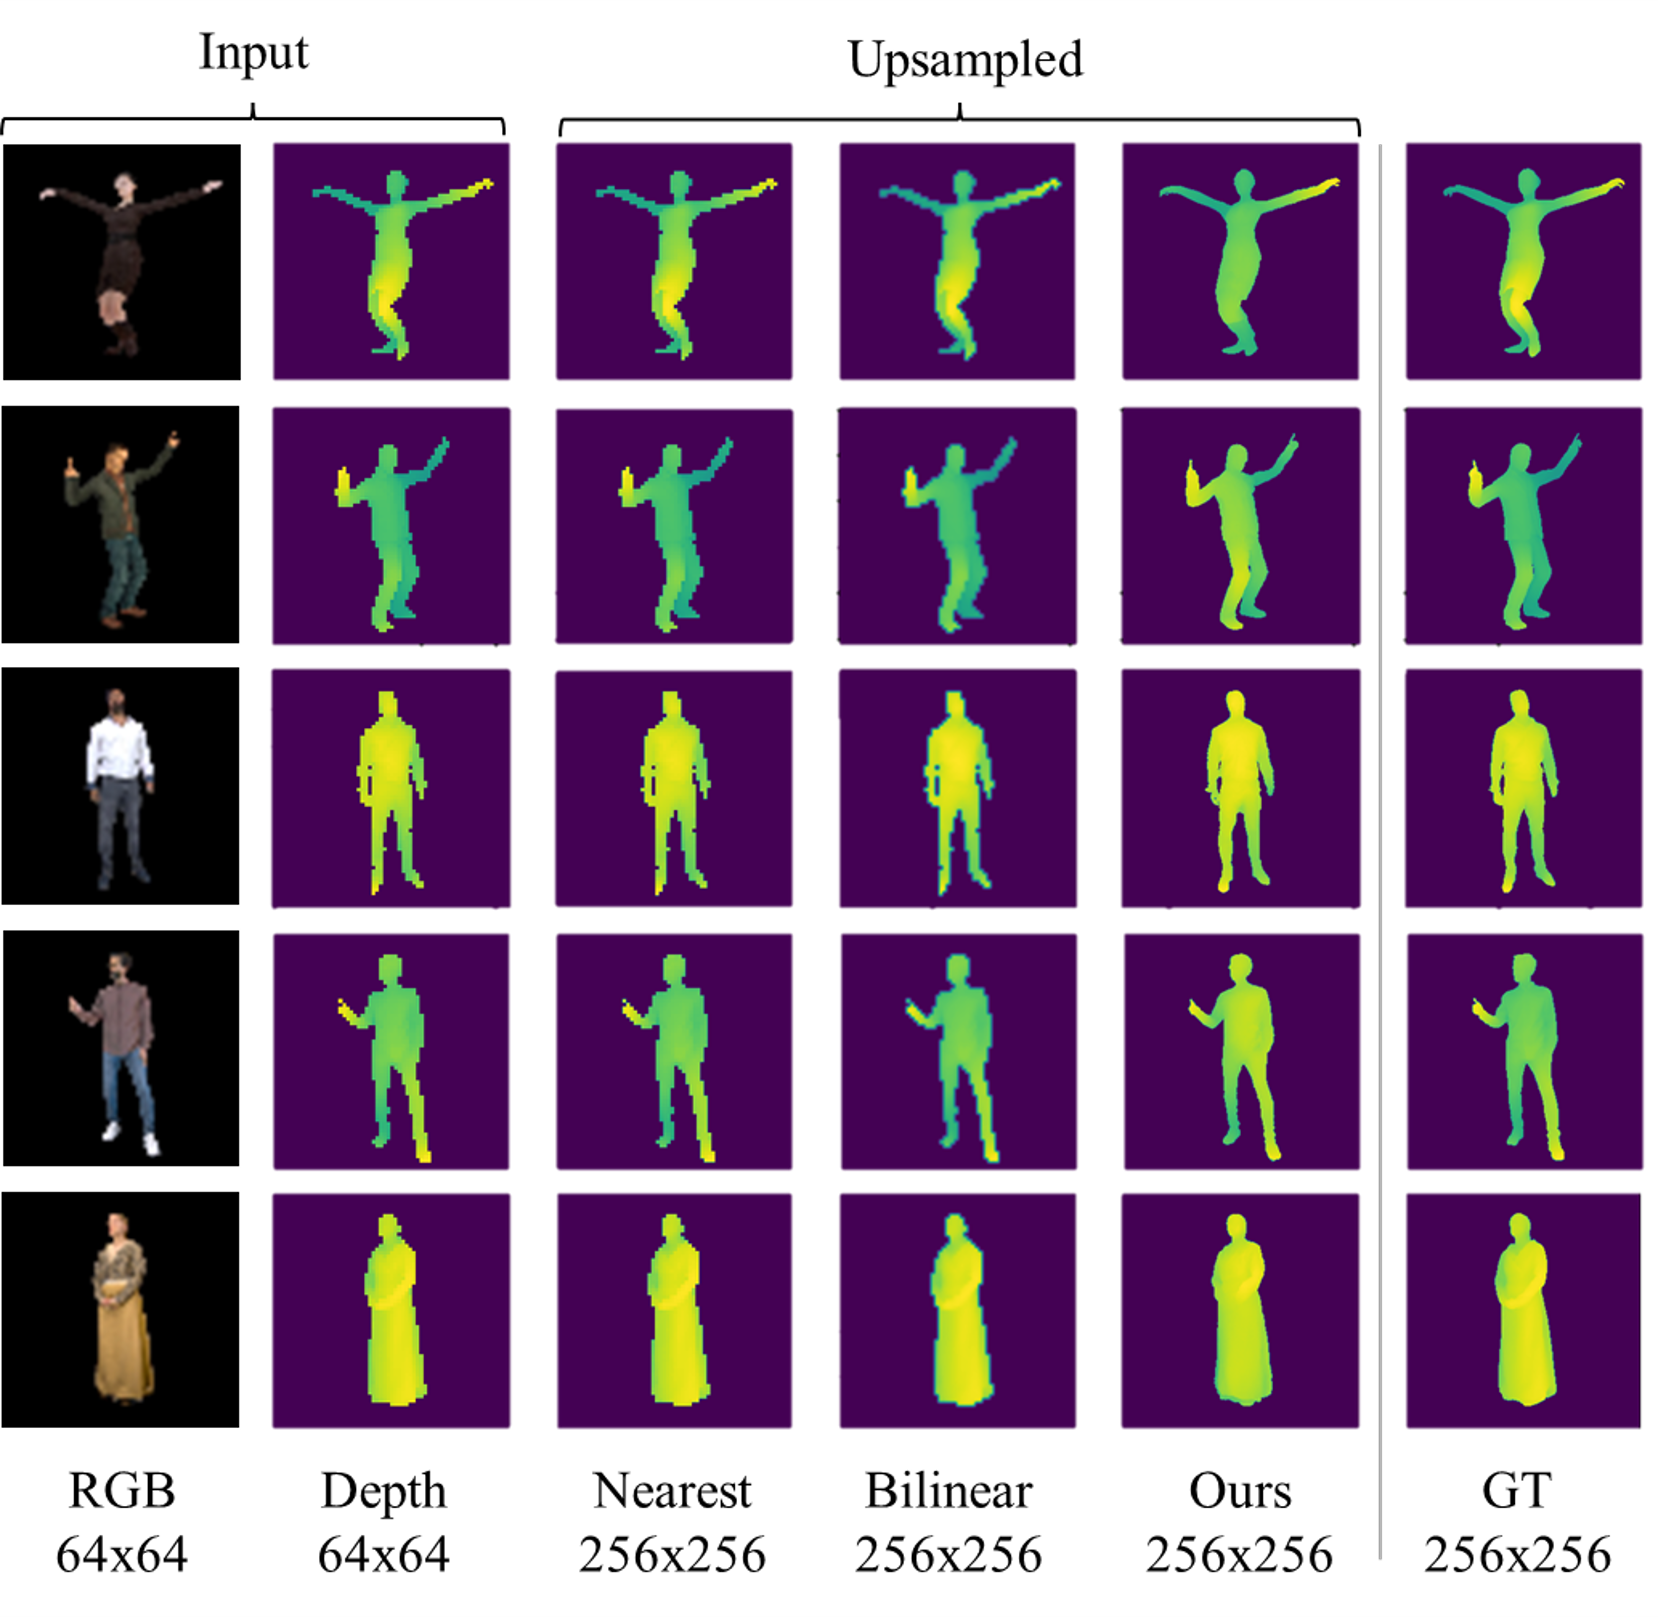
\includegraphics[width=0.99\linewidth]{illustrations/superres_method_comparison.png}
  \caption{Comparison of our diffusion based depth super-resolution model sr121 against other resampling techniques and the ground truth.}
  \label{fig:superres_method_comparison}
\end{figure}

\begin{figure}[t]
  \centering
  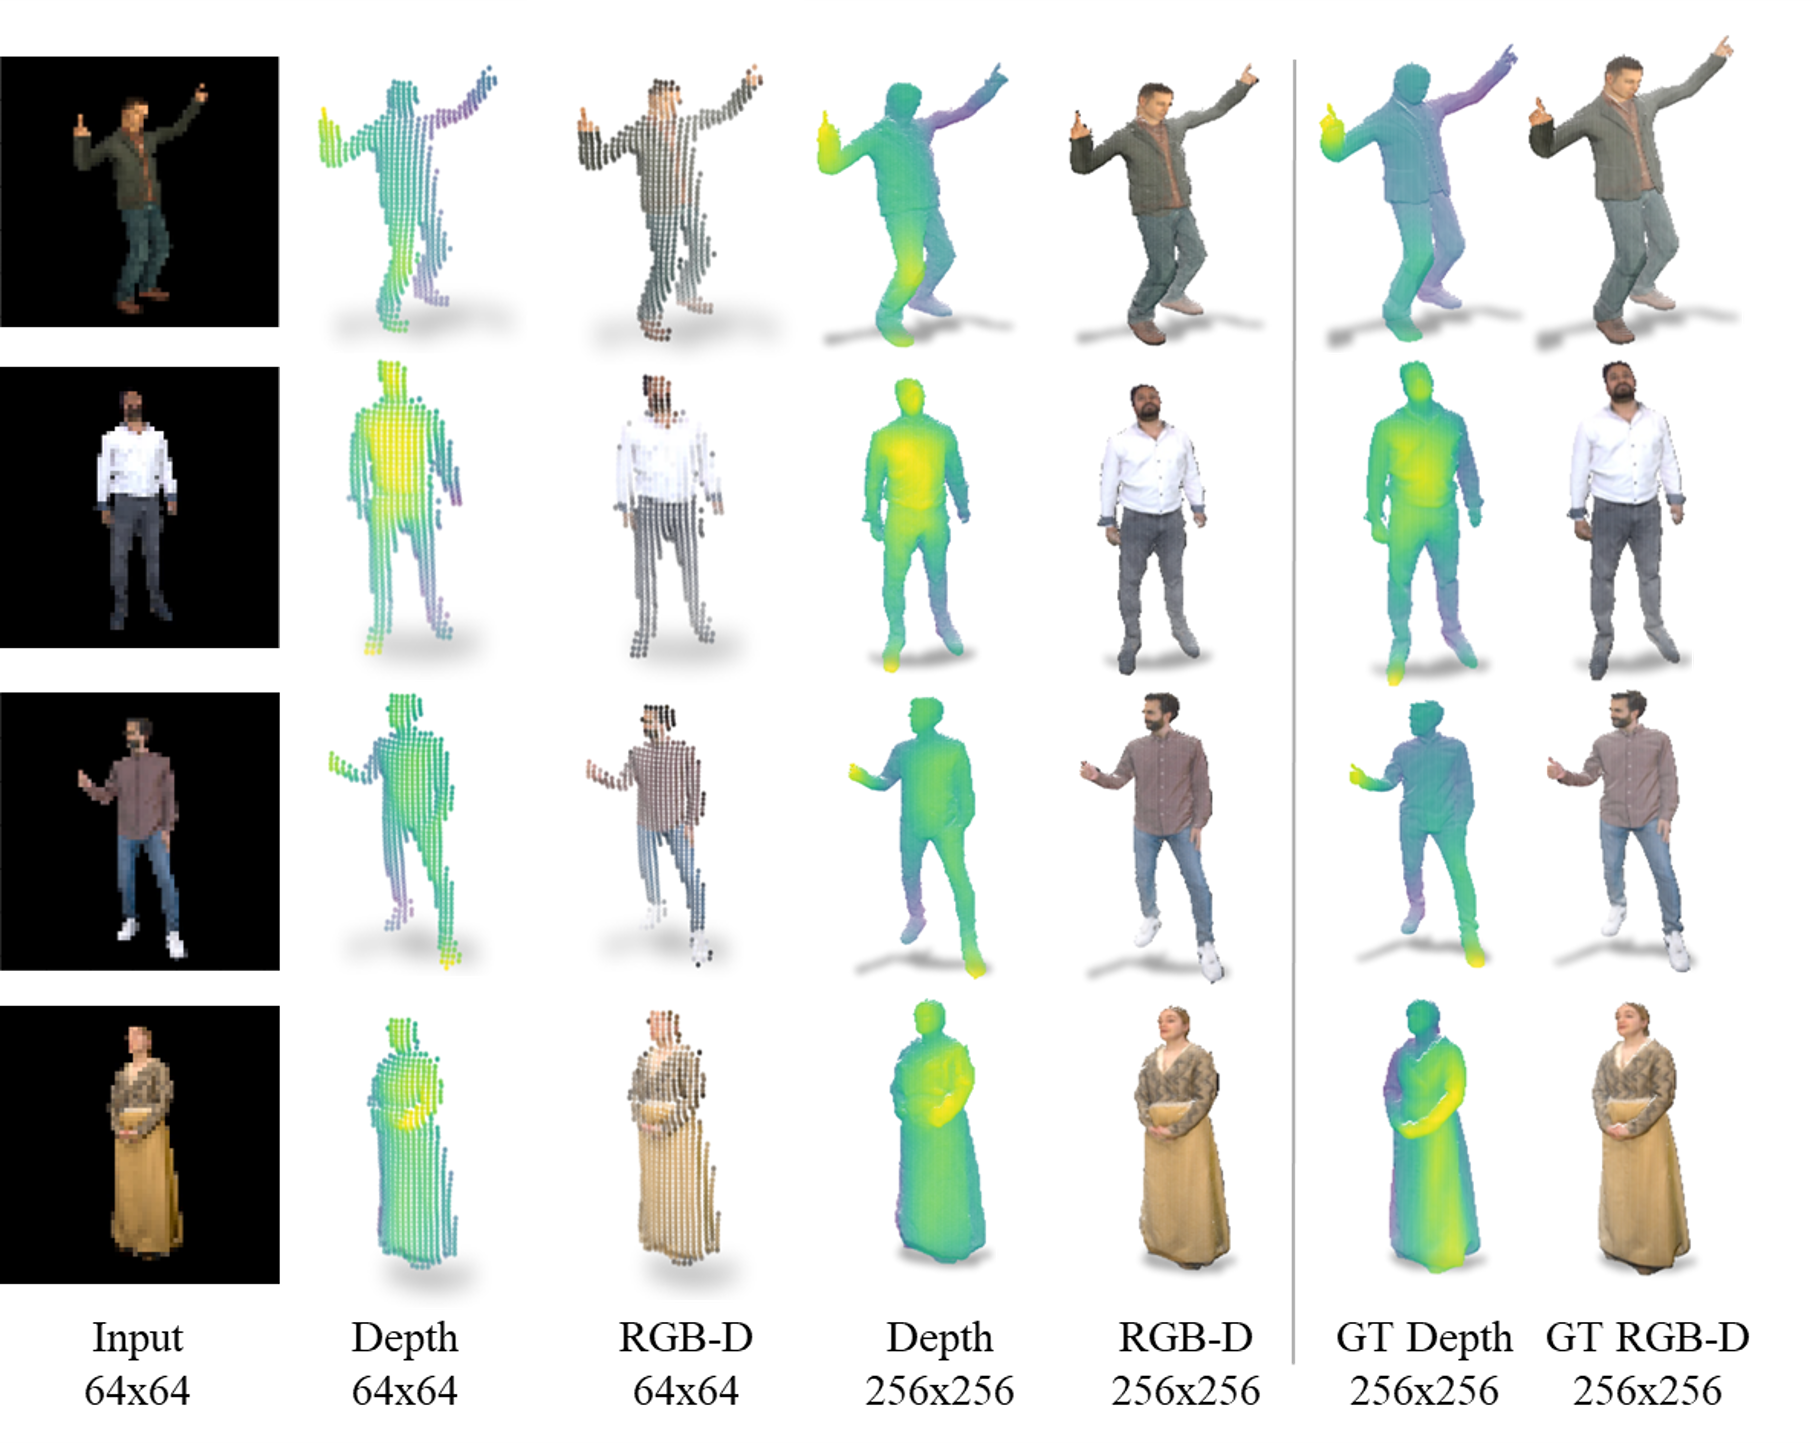
\includegraphics[width=0.99\linewidth]{illustrations/superres_pc.png}
  \caption{Input and output of our \modelname{} framework at various stages compared to the ground truth. We use model dd10 for the depth diffusion and sr121 for the depth super-resolution}
  \label{fig:rgb_d_fusion_pipeline_output}
\end{figure}

\begin{figure*}[t]
  \centering
  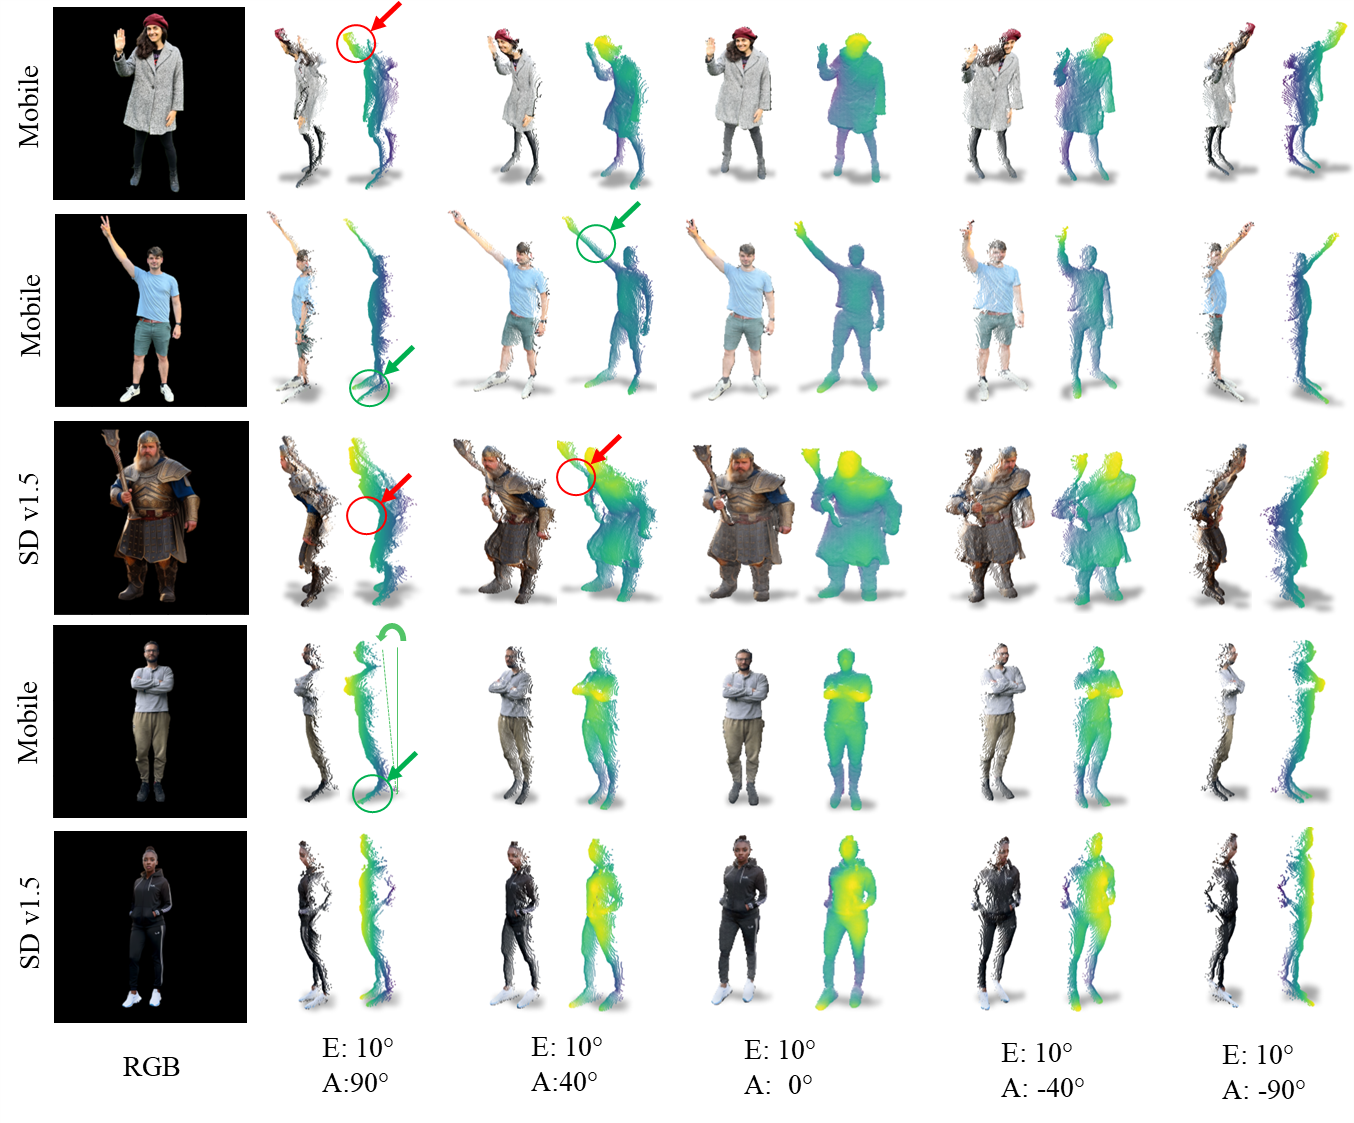
\includegraphics[width=0.99\linewidth]{illustrations/in_the_wild.png}
  \caption{Perspective depth and RGB-D output of our \modelname{} framework conditioned on RGB images obtained from either mobile cameras or images generated with stable diffusion v1.5. Results are illustrated from different viewpoints, i.e. different elevation angles E and azimuth angles A. Errors and distortions are highlighted in red, while distortions related to perspective projection are highlighted in green.}
  \label{fig:in_the_wild}
\end{figure*}

We further test our \modelname{} framework on "in the wild predictions" where we condition the depth diffusion process on RGB images obtained from different mobile cameras and RGB images generated using stable diffusion v1.5 \citep{rombach_high-resolution_2022}. We aim to investigate how well the framework generalizes to RGB images from a different data domain. Some results are shown in Fig. \ref{fig:in_the_wild} and further results are provided in the appendix in Fig. \ref{fig:rgb_d_fusion_wild_rgbd_1} and Fig. \ref{fig:rgb_d_fusion_wild_rgbd_2} for images obtained from a mobile camera and Fig. \ref{fig:rgb_d_fusion_wild_rgbd_3} for images generated using stable diffusion v1.5.

We observe that for most cases a plausible perspective depth is generated, showing typical distortions such as the subject being tilted towards the camera and lengthen extremities like feet and arms. In some cases the predictions show implausible depths. The super-resolution model on the other hand successfully increases the resolution even of subjects with such implausible depth maps indicating it is robust against domain shifts and solely focusing on increasing the depth maps resolution, which is desirable.
We hypothesize that the implausible depth is caused by a large domain gap between the input data and the training data in at least two aspects. First, a domain gap related to the subject's characteristics like pose, cloths, carried objects as well as lighting and colors in the image. Second, the position and intrinsic parameters of the camera that captured the image are significantly different as those used for rendering our dataset.